% AI-translated into English: printed 232--241.
% Principal PDF239--248; Google PDF243--252.
\begingroup
\clearpage
\noindent232\hfill\textsc{Trigonometric Point Determination.}\hfill\mbox{}\par\medskip
With respect to a second point of known position, let $\varphi'$, $\alpha'$, $\beta'$, and with respect to a third, let $\varphi''$, $\alpha''$, $\beta''$, and so on, have the same meanings as $\varphi$, $\alpha$, $\beta$ have with respect to the first.

If the angles at the station to be determined were measured in a single set with a theodolite without repetition, by directing the telescope successively at the various known points while the instrument remained fixed, then, if $h$, $h'$, $h''$, and so on denote the angle readings, the expressions
\[
\begin{gathered}
\varphi-h+\alpha\,\mathrm dx+\beta\,\mathrm dy\\
\varphi'-h'+\alpha'\mathrm dx+\beta'\mathrm dy\\
\varphi''-h''+\alpha''\mathrm dx+\beta''\mathrm dy\\
\text{and so on}
\end{gathered}
\]
would all take the same value upon substituting the true values of $\mathrm dx$ and $\mathrm dy$ if the observations were absolutely exact. Thus, by equating three of these expressions, one would obtain the values of $\mathrm dx$ and $\mathrm dy$ by elimination. If only three known points were observed, this is as far as one can go. If there are more, the errors in the angle measurements are most fully adjusted by adding all the expressions above, dividing the sum by their number, setting the difference between this quotient and each individual expression $=0$, and treating these equations according to the familiar rule of the method of least squares.

If the angles were measured independently of one another, each measurement immediately gives an equation between the unknown quantities $\mathrm dx$ and $\mathrm dy$. All these equations are then to be combined by the method of least squares, allowing, if desired, for any difference in the reliability of the angles. If, for example, the angle between the first and second points were found to be $=i$, that between the second and third $=i'$, and so on, always reckoned from left to right, one would have the equations
\[
\begin{gathered}
\varphi'-\varphi-i+(\alpha'-\alpha)\mathrm dx+(\beta'-\beta)\mathrm dy=0\\
\varphi''-\varphi'-i'+(\alpha''-\alpha')\mathrm dx+(\beta''-\beta')\mathrm dy=0\\
\text{and so on}
\end{gathered}
\]

\clearpage
\noindent\mbox{}\hfill\textsc{Trigonometric Point Determination.}\hfill233\par\medskip
If these angle measurements are equally reliable, one forms two normal equations from these equations. The first is formed by multiplying the equations in order by the respective coefficients of $\mathrm dx$, that is, the first by $\alpha'-\alpha$, the second by $\alpha''-\alpha'$, and so on, and adding them all. The second is formed by doing the same with the coefficients of $\mathrm dy$ and again adding them. If the angle measurements are of unequal precision and, for example, the first is based on $\mu$ repetitions, the second on $\mu'$, and so on, the equations must in both cases also be multiplied by the respective numbers $\mu$, $\mu'$, and so on before addition. From the two normal equations thus obtained, $\mathrm dx$ and $\mathrm dy$ are then found by elimination. (These rules are added solely for those unfamiliar with the method of least squares, who may also need to be reminded that in these multiplications the algebraic signs of $\alpha'-\alpha$, and so on, must be carefully observed.) Finally, I would add that \textls[100]{only} the errors in the angle measurements are to be adjusted here, since the coordinates of the known points are regarded as \textls[100]{exact}.

I shall illustrate these rules for the second case using the angles measured on Holkensbastion near Copenhagen that you sent me, although the last assumption mentioned appears to hold with insufficient accuracy in this instance. At such small distances, slight errors of a few tenths of a foot in the given coordinates have a much greater effect than errors in the angle measurements. It is therefore hardly surprising that even after the angles have been adjusted as far as possible, differences remain that greatly exceed what can be supposed possible in the observations of the angles. For the present purpose of giving an example of the calculation, however, this need be of no consequence.
\begin{center}
Angles on Holkensbastion\textsuperscript{*)}.
\end{center}
\begin{center}
\begin{tabular}{lrrr}
Friedrichsberg---Petri&$73^\circ$&$35'$&$22''{,}8$\\
Petri---Erlösersthurm&104&57&$33{,}0$
\end{tabular}
\end{center}
\vfill
\noindent\rule{4cm}{.4pt}\par
{\footnotesize *) The coordinates of the points and the angles on Holkensbastion are both based on measurements by Captain von \textsc{Caroc}.\quad $S$\textit{[chumacher].}\par}
\medskip\noindent{\small IX.}\hfill30\hspace*{2cm}

\clearpage
\noindent234\hfill\textsc{Trigonometric Point Determination.}\hfill\mbox{}\par\medskip
\begin{center}
\begin{tabular}{lrrr}
Erlösersthurm---Friedrichsberg&$181^\circ$&$27'$&$5''{,}0$\\
Friedrichsberg---Frauenthurm&80&37&$10{,}8$\\
Frauenthurm---Friedrichsthurm&101&11&$50{,}8$\\
Friedrichsthurm---Friedrichsberg&178&11&$1{,}5$.
\end{tabular}
\end{center}
\begin{center}
Coordinates reckoned from the Copenhagen Observatory, in Paris feet.
\end{center}
\begin{center}
\begin{tabular}{lrr}
Petri&$+487{,}7$&$+1007{,}7$\\
Frauenthurm&$+710{,}0$&$+684{,}2$\\
Friedrichsberg&$+2430{,}6$&$+8335{,}0$\\
Erlösersthurm&$+2940{,}0$&$-3536{,}0$\\
Friedrichsthurm&$+3059{,}3$&$-2231{,}2$.
\end{tabular}
\end{center}
The following were adopted as approximate coordinates of the observing station:
\[
x=+2836{,}44,\qquad y=+444{,}33.
\]
These gave the azimuths:
\[
\begin{array}{lrrr@{\;}l}
\text{Petri}&166^\circ&30'&42''{,}56&+19{,}92\mathrm dx+83{,}04\mathrm dy\\
\text{Frauenthurm}&173&33&50{,}54&+10{,}80\mathrm dx+95{,}78\mathrm dy\\
\text{Friedrichsberg}&92&56&39{,}46&+26{,}07\mathrm dx+\phantom01{,}34\mathrm dy\\
\text{Erlösersthurm}&271&29&25{,}38&-51{,}79\mathrm dx-\phantom01{,}35\mathrm dy\\
\text{Friedrichsthurm}&274&45&41{,}39&-76{,}56\mathrm dx-\phantom06{,}38\mathrm dy.
\end{array}
\]
The calculated angle Friedrichsberg---Petri is therefore
\[
73^\circ34'3''{,}10-6{,}15\mathrm dx+81{,}70\mathrm dy,
\]
which, when compared with the observed angle, gives the equation
\[
-79{,}70-\phantom06{,}15\mathrm dx+\phantom081{,}70\mathrm dy=0
\]
The other five equations are obtained in the same way
\[
\begin{array}{r@{\;}r@{\;}r@{\;}l}
+69{,}82&-71{,}71\mathrm dx&-84{,}39\mathrm dy&=0\\
+9{,}08&+77{,}86\mathrm dx&+2{,}69\mathrm dy&=0\\
+0{,}28&-15{,}27\mathrm dx&+94{,}44\mathrm dy&=0\\
+0{,}05&-87{,}36\mathrm dx&-102{,}16\mathrm dy&=0\\
-3{,}43&+102{,}63\mathrm dx&+7{,}72\mathrm dy&=0.
\end{array}
\]
\clearpage
\noindent\mbox{}\hfill\textsc{Trigonometric Point Determination.}\hfill235\par\medskip
Combining these six equations and assigning equal reliability to the observations gives the two normal equations
\[
\begin{aligned}
+29640\mathrm dx+14033\mathrm dy&=+\phantom04170\\
+14033\mathrm dx+33219\mathrm dy&=+12384,
\end{aligned}
\]
and from these the values
\[
\mathrm dx=-0{,}04,\qquad\mathrm dy=+0{,}39,
\]
or the corrected coordinates of Holkensbastion
\[
+2836{,}40\quad\text{and}\quad+444{,}72.
\]
The differences that remain between the calculated and observed angles after substitution of these values of $\mathrm dx$ and $\mathrm dy$ are still much too large to be attributed to the measurements. They show, as remarked above, that the coordinates of the known points could not be relied on to tenths of a foot, so that in this case the correction itself naturally remains somewhat doubtful.

The approximate coordinates of Holkensbastion used as the basis for this calculation were computed by the \textls[100]{direct} method from the fourth and fifth of the angles above. Although this direct method may be regarded as a fairly thoroughly treated subject, for completeness I give it here as well, in the form in which I usually apply it.

Let $a$, $b$ be the coordinates of the first known point (which may be chosen at will from the three known points). Write the coordinates of the second in the form
\[
a+R\cos E,\qquad b+R\sin E
\]
and those of the third in the same form:
\[
a+R'\cos E',\qquad b+R'\sin E'.
\]
Denote the sought coordinates of the observation point by
\[
a+\rho\cos\varepsilon,\qquad b+\rho\sin\varepsilon.
\]
Furthermore, let the angle observed here between the first and second
\vfill\noindent\hfill30\textsuperscript{$\ast$}\hspace*{2cm}

\clearpage
\noindent236\hfill\textsc{Trigonometric Point Determination.}\hfill\mbox{}\par\medskip
\noindent points be $=M$, and that between the first and third be $=M'$. I assume that these angles are taken from left to right and that any angle thus greater than $180^\circ$ has first been reduced by $180^\circ$. Equivalently, if an angle taken in the reverse order was less than $180^\circ$, its supplement to $180^\circ$ has been taken instead\textsuperscript{*)}. I further set
\[
\begin{array}{rcl@{\qquad}rcl}
\frac R{\sin M}&=&n,&\frac{R'}{\sin M'}&=&n'\\[5pt]
E-M&=&N,&E'-M'&=&N'
\end{array}
\]
(where, if necessary, $360^\circ$ is first added).

With these assumptions one has the two equations
\[
\rho=n\sin(\varepsilon-N),\qquad\rho=n'\sin(\varepsilon-N'),
\]
which, when written as
\[
\frac1n=\frac1\rho\sin(\varepsilon-N),\qquad\frac1{n'}=\frac1\rho\sin(\varepsilon-N'),
\]
fall under the problem in Theor. Mot. C. C. p.~82 [**)]. One of the solutions given there leads to the following rule:

I assume that $n'$ is greater than, or at least as large as, $n$. This is permissible, since the choice of which point is to be considered the second or the third is arbitrary. Let
\[
\begin{gathered}
\frac n{n'}=\operatorname{tang}\zeta\\[5pt]
\frac{\operatorname{tang}\frac12(N'-N)}{\operatorname{tang}(45^\circ-\zeta)}=\operatorname{tang}\psi.
\end{gathered}
\]
Then
\[
\varepsilon=\tfrac12(N+N')+\psi,
\]
and once $\varepsilon$ has been found, $\rho$ is calculated by one of the formulas above, or, better, by both.

In our example, taking the Frauenthurm as the first point, Friedrichsberg provisionally as the second, and the Friedrichsthurm as the third, we have:
\vfill
\noindent\rule{4cm}{.4pt}\par
{\footnotesize
*) The purpose is to make the quantities $n$, $n'$ that follow always positive, so that less attention need be paid to algebraic signs.\par
[**) Volume VII, page 100.]\par}

\clearpage
\noindent\mbox{}\hfill\textsc{Trigonometric Point Determination.}\hfill237\par\medskip
\[
\begin{array}{rcl@{\qquad}rcl}
a&=&+710{,}0&b&=&+684{,}2\\
E&=&77^\circ19'31''{,}91&E'&=&308^\circ51'45''{,}78\\
\log R&=&3{,}894\,4206&\log R'&=&3{,}573\,3549\\
M&=&99^\circ22'49''{,}20&M'&=&101^\circ11'50''{,}80\\
\multicolumn{3}{c}{\text{(see the note above)}}&&&\\
N&=&337^\circ56'42''{,}71&N'&=&207^\circ39'54''{,}98\\
\log n&=&3{,}900\,2671&\log n'&=&3{,}581\,7019.
\end{array}
\]
Since $n>n'$ here, we reverse the order and set
\[
\begin{array}{rcl@{\qquad}rcl}
N&=&207^\circ39'54''{,}98&N'&=&337^\circ56'42''{,}71\\
\log n&=&3{,}581\,7019&\log n'&=&3{,}900\,2671.
\end{array}
\]
We then find
\[
\zeta=25^\circ39'3''{,}49,\qquad
\psi=80^\circ45'31''{,}50,\qquad
\varepsilon=353^\circ33'50''{,}34
\]
and $\log\rho=3{,}330\,3996$, with coordinates $+2836{,}444$ and $+444{,}327$ for Holkensbastion.
\vspace{1cm}
\begin{center}\rule{4cm}{.4pt}\end{center}

\clearpage
\noindent238\hfill\textsc{Posthumous Papers.}\hfill\mbox{}\par
\vspace{1.5cm}
\begin{center}{\Large\textls[150]{POSTHUMOUS PAPERS.}}\end{center}
\bigskip
\begin{center}[7.]\\[5pt]
[Determination of the Position of Point X by Observing the Angles $\alpha$ and $\beta$ Between 3 Given Points $A$, $B$, $C$.]
\end{center}
[From
\[
\frac{BA}{BX}.\frac{BX}{BC}.\frac{BC}{BA}=1
\]
it follows that
\[
\frac{\sin XCB}{\sin BAX}=\frac{\sin C}{\sin A}=\frac{c\sin\beta}{a\sin\alpha}\,\bigg]
\]
\begin{center}
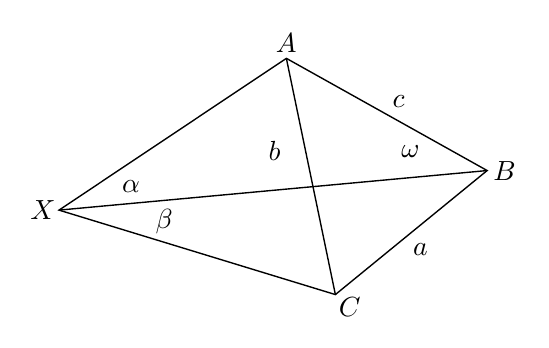
\begin{tikzpicture}[x=.75cm,y=.75cm,line width=.5pt]
\coordinate (X) at (0,0);
\coordinate (A) at (3.85,2.57);
\coordinate (B) at (7.25,.67);
\coordinate (C) at (4.68,-1.43);
\draw (X)--(A)--(B)--(C)--cycle;
\draw (X)--(B) (A)--(C);
\node[above,inner sep=2pt] at (A) {$A$};
\node[right,inner sep=2pt] at (B) {$B$};
\node[below right,inner sep=1pt] at (C) {$C$};
\node[left,inner sep=1pt] at (X) {$X$};
\node at (1.22,.40) {$\alpha$};
\node at (1.78,-.19) {$\beta$};
\node at (3.65,1.00) {$b$};
\node at (5.75,1.84) {$c$};
\node at (5.95,1.00) {$\omega$};
\node at (6.12,-.66) {$a$};
\end{tikzpicture}
\end{center}
[If one sets
\[
\begin{gathered}
180^\circ-A=]\ \alpha+\omega=\lambda,\qquad [C=360^\circ-(A+\varepsilon),]\\
\alpha+\beta+B=\varepsilon\\[5pt]
\operatorname{tang}\varphi=\sqrt{\frac{c\sin\beta}{a\sin\alpha\cos\varepsilon}},
\end{gathered}
\]
then
\[
\begin{gathered}
\operatorname{tang}\lambda=\operatorname{tang}\varepsilon\cos\varphi^2,\\
BX=\frac{c\sin\lambda}{\sin\alpha}.
\end{gathered}
\]
\clearpage
\noindent\mbox{}\hfill\textsc{Trigonometric Point Determination.}\hfill239\par\medskip
\begin{center}[8.]\\[5pt]Orientation of the Plane Table.\rlap{\hspace{.12em}\raisebox{1.15ex}{\scriptsize,}}\end{center}
Three places $A$, $B$, $C$ are represented on the p[lane] t[able] by $a$, $b$, $c$. The straight lines $Aa$, $Bb$, $Cc$ intersect one another at the points $\alpha$, $\beta$, $\gamma$.

The perpendiculars erected at $b$ to $ab$ and at $\gamma$ to $a\gamma$ intersect at $e$. The perpendiculars at $c$ to $ac$ and at $\beta$ to $a\beta$ intersect at $f$. Join $e$ and $f$ and from $a$ drop the perpendicular $aM$ to this line. Then $M$ is the station on the plane table.
\bigskip
\begin{center}[9.]\\[5pt]A Problem in Practical Geometry.\end{center}
$A$, $B$, $C$, $D$ are four points in a horizontal plane. The points $B$, $C$, $D$ lie on a straight line and
\[
BC=CD.
\]
Let the azimuths of the lines be
\[
\begin{array}{l@{\;}l}
DB\ .\ .\ .\ .&f\\
AB\ .\ .\ .\ .&f+g-\delta\\
AC\ .\ .\ .\ .&f+g-x\\
AD\ .\ .\ .\ .&f+g+\delta.
\end{array}
\]
\begin{center}
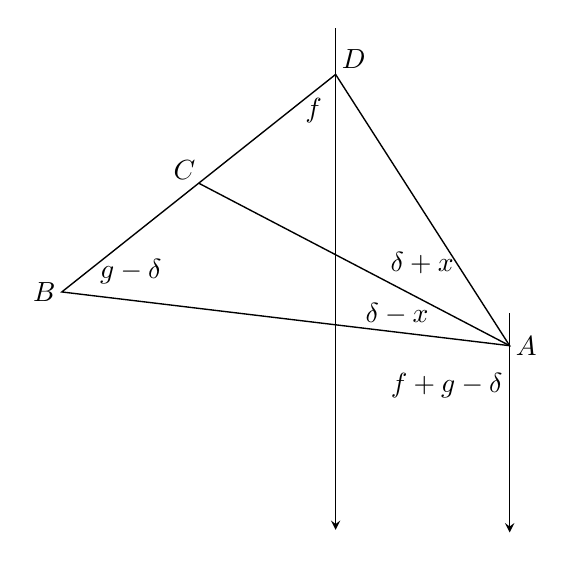
\begin{tikzpicture}[x=.65cm,y=.65cm,line width=.5pt]
\coordinate (B) at (0,0);
\coordinate (D) at (5.35,4.25);
\coordinate (C) at (2.675,2.125);
\coordinate (A) at (8.75,-1.05);
\draw (B)--(D)--(A)--cycle;
\draw (C)--(A);
\draw[->,>=stealth] (5.35,5.15)--(5.35,-4.65);
\draw[->,>=stealth] (8.75,-.42)--(8.75,-4.7);
\node[left,inner sep=2pt] at (B) {$B$};
\node[above left,inner sep=1pt] at (C) {$C$};
\node[above right,inner sep=2pt] at (D) {$D$};
\node[right,inner sep=2pt] at (A) {$A$};
\node at (1.35,.39) {$g-\delta$};
\node at (4.92,3.55) {$f$};
\node at (7.04,.57) {$\delta+x$};
\node at (6.55,-.44) {$\delta-x$};
\node at (7.52,-1.83) {$f+g-\delta$};
\end{tikzpicture}
\end{center}

\clearpage
\noindent240\hfill\textsc{Remarks.}\hfill\mbox{}\par\medskip
\[
\bigg[\frac{AC}{BC}=\frac{AC}{CD}\quad\text{or}\quad
\frac{\sin(g-\delta)}{\sin(\delta-x)}=\frac{\sin(g+\delta)}{\sin(\delta+x)}.\bigg]
\]
Then
\[
\begin{gathered}
\operatorname{tang}x=\frac{\operatorname{tang}\delta^2}{\operatorname{tang}g},\\[6pt]
\sin x=\frac{\sin\delta^2\cos(g-x)}{\sin g},
\end{gathered}
\]
or, approximately,
\[
x=206265''\sin\delta^2\operatorname{cotang}g.
\]
\bigskip
\begin{center}\rule{3cm}{.4pt}\\[6pt]\textsc{Remarks.}\end{center}
\begingroup\footnotesize
Notes [1] and [9], [3] and [4], and [8] were taken from 3 different notebooks. Notes [2] and [7] are entered on the last pages of logarithm tables. Note [5] comes from a calculation sheet for the Hanoverian arc measurement.

The formulas of Art.~[2], which are also used in Art.~[3], can be derived as follows. Let $x$, $y$ be the coordinates of the point to be determined, $x_0$, $y_0$ the coordinates of its approximate position, $a$, $b$, $a'$, $b'$, $a''$, $b''$ the coordinates of the observing stations, and $r$, $r'$, $r''$ the distances of these stations from the point $(x_0,y_0)$. Then by differentiating the equation
\[
\operatorname{tang}(A+\alpha)=\frac{y_0-b}{x_0-a},
\]
and setting $\mathrm dx_0=x-x_0$, $\mathrm dy_0=y-y_0$, $A+\alpha+\mathrm d(A+\alpha)=A+\delta A$, one obtains the error equation:
\[
\delta A-\alpha=-\sin A.\frac{x-x_0}{r}+\cos A.\frac{y-y_0}{r}.
\]
Similarly one obtains
\[
\delta A'-\alpha'=-\sin A'.\frac{x-x_0}{r'}+\cos A'.\frac{y-y_0}{r'}
\]
and
\[
\delta A''-\alpha''=-\sin A''.\frac{x-x_0}{r''}+\cos A''.\frac{y-y_0}{r''}.
\]
Eliminating $x-x_0$, $y-y_0$ gives the condition equation:
\[
r\sin(A'-A'').(\delta A-\alpha)+r'\sin(A''-A).(\delta A'-\alpha')+r''\sin(A-A').(\delta A''-\alpha'')=0
\]
or
\[
l.\delta A+l'.\delta A'+l''.\delta A''=l\alpha+l'\alpha'+l''\alpha''.
\]
Now if, taking this into account, one reduces
\[
g.\delta A^2+g'.\delta A'^2+g''.\delta A''^2\quad\text{to a minimum},
\]
then
\par\endgroup

\clearpage
\noindent\mbox{}\hfill\textsc{Trigonometric Point Determination.}\hfill241\par\medskip
\begingroup\footnotesize
\[
\delta A=\frac{lk}{g},\qquad\delta A'=\frac{l'k}{g'},\qquad\delta A''=\frac{l''k}{g''};
\]
\[
k=\frac{l\alpha+l'\alpha'+l''\alpha''}{\dfrac{ll}{g}+\dfrac{l'l'}{g'}+\dfrac{l''l''}{g''}}.
\]
Hence
\[
y-b=(x-a)\operatorname{tang}(A+\delta A)=(x-a)\operatorname{tang}A+\frac{r.\delta A}{\cos A}
=(x-a)\operatorname{tang}A+\frac{rlk}{g\cos A}.
\]
A few small errors in the numerical example under [3] have been corrected, so the coordinate values obtained here for York differ somewhat from those given in the coordinate register, Volume IV, p.~436.

A small oversight has likewise been corrected in the example of forward intersection under [5]. The azimuths observed at the fixed points and the coordinates are also given in the »Abrissen u.\,s.\,w.«, Volume IV, pp.~454, 456 and 457.

To determine secondary points, \textsc{Gauss} and the officers assigned to him usually used the procedure of Art.~[5]. The calculations, however, were carried out almost entirely by \textsc{Gauss} alone, in the manner indicated. The report on the work for 1830 to the Hanoverian ministry reads: »In the trigonometric survey here I have so far undertaken this part of the work [reducing the measurements to results] entirely on my own. My reports on the work of 1828 and 1829 give an overview of the extent of what was accomplished in those years. Without going into lengthy details here, I must mention that I was able to carry out the reduction only by devoting to it \textls[100]{all} the time left to me by my immediate official duties.« In the report submitted to the ministry on 8~February 1838, \textsc{Gauss} says: »A trigonometric survey requires two quite different kinds of work: making the measurements at the relevant stations in the field, and reducing them to results by combination and calculation indoors. I have so far undertaken the second part of the work entirely on my own.« His son, Lieutenant J.~\textsc{Gauss}, helped him with this for only two months during the winter of 1830/31. Professor \textsc{Goldschmidt} also appears to have helped in the last years of the Hanoverian land survey. The following remarks are taken from a »geodätischen Calcül nach \textsc{Gauss}« that Goldschmidt drew up in 1835 and intended as a »brief account based on private communications from \textsc{Gauss}«:

»In establishing the secondary points, we begin by determining those that can be determined \textls[100]{precisely} from the points of the principal triangulation alone, so that 1) the directions do not intersect at angles that are too acute and 2) one is certain that the azimuths given really refer to the point in question, since in extensive operations names are unfortunately confused only too often. If, however, the point has been determined from more than 2 principal points, or measurements have been made at the point itself, such a confusion is hardly possible. To establish these secondary points and obtain precise results, one takes into account all the points of the principal triangulation as well as the intersections made toward and from other secondary points already determined. There are 3 unknown quantities here, namely the coordinates of the point and the orientation at that point. These elements are then calculated for the remaining secondary points as well. If it should later be thought advisable to introduce new secondary points, perhaps because the advisability of introducing them was overlooked in the original plan, there is still no need to go to the stations from which the new
\par\endgroup
\vfill\noindent{\small IX.}\hfill31\hspace*{2cm}
\endgroup
% Continues on printed 242 with "points could be intersected".
